%\section{Werkzeuge und Technologien}
%\label{sec:werkzeuge-und-technologien}

%\textit{Basierend auf dem Grundwissen über die Methoden und Praktiken, soll nun der Stand der Technik erörtert werden. Hierbei sollen Werkzeuge und Technologien und ihre Ansätze hervorgehoben werden und mit Hilfe welcher Methoden sie welches Ziel erreichen.}
%
%\textit{Wie in der Zielsetzung definiert sollen hier zwei bis drei Technologien näher vorgestellt werden.}
%
%\textit{Weiterhin könnte beleuchtet werden, wie ähnliche Herausforderungen bei anderen „Fat-Client“-Lösungen (also nicht SPAs) angegangen werden, und kann man hier vielleicht etwas lernen oder übertragen (und wenn nicht, warum nicht)?}

Um die gewünschte Lösung, also ein Proof-of-Concept, zu erstellen, ist zuvor der Stand der Technik zu erörtern. In diesem Abschnitt wird versucht einen repräsentativen Durchschnitt aktueller Technologien vorzustellen, diese zu kategorisieren und dann auf zuvor definierten Kriterien zu bewerten.

\subsection{Recherche}

Damit das gewünschte Ziel dieses Abschnitts erreicht wird, wurde neben verfügbarer Literatur auch auf etablierte Plattformen im Gebiet der Gegenüberstellung von Technologien gesetzt. Speziell wurden hierbei Gartner\footnote{Gartner ist ein global agierendes Forschungs- und Beratungsunternehmen im Bereich der IT \cite{GartnerDefinition}} sowie StackShare\footnote{StackShare (\url{https://stackshare.io}) ist eine Vergleichsseite für Entwicklerwerkzeuge und Technologien, die auf Basis von Nutzereingaben Vergleiche erzeugt \cite{StackshareDefinition}} herangezogen. Die identifizierten Technologien werden im nachfolgenden Abschnitt veranschaulicht und kategorisiert. 

Mithilfe von Gartners \enquote{Magic Quadrant for APM} \cite{GartnerMagicQuadrantForAPM} konnte festgestellt werden, dass folgende APM-Werkzeuge zu den führenden Technologien dieser Kategorie angehören: AppDynamics \cite{AppDynamics}, Dynatrace (ehemals ruxit) \cite{Dynatrace}, New Relic \cite{NewRelic}, Broadcom DX APM \cite{BroadcomDXAPM}, Splunk APM \cite{SplunkAPM} sowie Datadog\cite{Datadog}. Bestätigt werden einige dieser Nennungen in der Bewertung bei StackShare \cite{StackShareAPM}, insbesondere New Relic und Datadog werden oft eingesetzt und positiv bewertet. Hinzukommend wird hierbei die Application Insights \cite{AzureApplicationInsights} des Azure Monitors von Microsoft in den Top 6 genannt.

Mart{\'i}nez \etal \cite{ComparisonOfE2ETestingToolsForMicroservices} fanden in ihrer Evaluierung von Werkzeugen bei der Unterstützung von E2E-Tests, dass die beiden OpenSource-Technologien Jaeger \cite{Jaeger} und Zipkin \cite{Zipkin} aktiv dabei helfen können Fehlerszenarien in Microservice-Architekturen besser nachzuvollziehen. Li \etal \cite{ServiceMeshChallengesStateOfTheArt} beschreiben, wie mit Prometheus \cite{Prometheus}, Jaeger, Zipkin und Fluentd \cite{Fluentd} eine Datenanalyse von Microservices ermöglicht werden kann. Weiterhin beschreiben Picoreti \etal \cite{MultilevelObservabilityInCloudOrchestration} eine Observability-Architektur, die auf Fluentd, Prometheus und Zipkin basiert.

Bei StackShares Gegenüberstellung von Error-Monitoring-Produkten \cite{StackShareExceptionMonitoring} stehen drei Technologie hervor: Sentry \cite{Sentry}, TrackJS \cite{TrackJS} sowie Rollbar \cite{Rollbar}. Sentry und TrackJS waren zudem auch bei der Gegenüberstellung der Monitoring-Lösungen \cite{StackShareMonitoring} gelistet.

StackShare bezeichnet Session-Replay als \enquote{User-Feedback-as-a-Service} und hierbei \cite{StackShareUserFeedbackAsAService} lassen sich ebenfalls drei etablierte Produkte identifizieren: Inspectlet \cite{Inspectlet}, FullStory \cite{FullStory} und LogRocket \cite{LogRocket}. Während jedoch Inspectlet und FullStory hauptsächlich darauf abzielen, dass die User-Experience nachvollzogen werden kann, konzentriert sich LogRocket auf technische Informationen, die für Entwickler von Bedeutung sind \cite{Webalyt}. Gartner bietet eine Übersicht \cite{GartnerWebAndMobileAppAnalytics} über Produkte im \enquote{Web and Mobile App Analytics Market} an, hierbei findet sich Google Analytics \cite{GoogleAnalytics}, Adobe Analytics \cite{AdobeAnalytics} sowie LogRocket auf den obersten Positionen.

\subsection{Übersicht}

Folgend werden in der \autoref{tab:technologie-uebersicht} die gefundenen Technologien näher veranschaulicht. Hierbei wird untersucht, welche Funktionalitäten die jeweilige Technologie vorweist, auf Basis der Produktbeschreiben der Hersteller. Genauer werden folgende, zuvor identifizierte, Funktionalitäten unterschieden und den Technologien zugeordnet: IM, ASM, RUM, Error-Monitoring, Log-Management, (Distributed-)Tracing sowie Session-Replay. Um anzugeben, wie der Funktionsumfang der jeweiligen Funktionalität ist, wird das Vorhandensein mit folgenden 4 Schlüsseln angegeben:

\begin{enumerate}
	\item \texttt{ja}: Die Funktionalität ist vorhanden und der Funktionsumfang entspricht der Definition.
	\item \texttt{ja(*)}: Die Funktionalität ist vorhanden, aber sie ist nicht vergleichbar umfangreich wie andere Technologien.
	\item \texttt{eingeschränkt}: Die Funktionalität ist nur unter bestimmten Voraussetzungen vorhanden oder ist nur teilweise implementiert.
	\item \textit{keine Angabe}: Die Funktionalität ist nicht vorhanden.
\end{enumerate}

\pagebreak

\hvFloat[rotAngle=90,nonFloat=true,capWidth=w]%
{table}%
{
\begin{tabular}{|p{2.25cm}|p{1.5cm}|p{2.0cm}|p{3.0cm}|p{3.0cm}|p{1.5cm}|p{2.5cm}|}
\hline
Technologie & APM & RUM & Error-Mo\-ni\-tor\-ing & Log-Management & Tracing & Session-Replay \\
\hline
Adobe Analytics &  & gruppiert & teils &  &  &  \\
\hline
AppDynamics & ja & gruppiert & ja &  & ja &  \\
\hline
Broadcom DX APM & ja &  & teils & ja & ja &  \\
\hline
DataDog & ja & gruppiert & ja & ja & ja &  \\
\hline
Dynatrace & ja & gruppiert & ja & ja & ja &  \\
\hline
Elastic Stack & möglich & möglich & möglich & ja &  &  \\
\hline
Fluentd &  &  &  & ja &  &  \\
\hline
FullStory &  & ja & teils &  &  & ja \\
\hline
Google Analytics &  & gruppiert & teils &  &  &  \\
\hline
Graylog &  &  &  & ja &  &  \\
\hline
Inspectlet &  & ja & teils &  &  & ja \\
\hline
Jaeger &  &  &  &  & ja &  \\
\hline
LogRocket &  & ja & ja & teils &  & ja \\
\hline
New Relic & ja & gruppiert & ja & ja & ja &  \\
\hline
Papertrail &  &  &  & ja &  &  \\
\hline
\end{tabular}
}
{Übersicht der untersuchten Technologien, Teil 1}
{tab:technologie-uebersicht-teil1}

\hvFloat[rotAngle=90,nonFloat=true,capWidth=w]%
{table}%
{
\begin{tabular}{|p{2.25cm}|p{1.5cm}|p{2.0cm}|p{3.0cm}|p{3.0cm}|p{1.5cm}|p{2.5cm}|}
\hline
Technologie & APM & RUM & Error-Mo\-ni\-tor\-ing & Log-Management & Tracing & Session-Replay \\
\hline
Prometheus & ja &  &  &  &  &  \\
\hline
Rollbar &  & bei \mbox{Fehlern} & ja &  &  & teils \\
\hline
Sentry &  & bei \mbox{Fehlern} & ja &  &  &  \\
\hline
Splunk APM (SignalFX) & ja &  & ja &  & ja &  \\
\hline
Splunk \mbox{Enterprise} & möglich & möglich & möglich & ja &  &  \\
\hline
TrackJS &  & bei \mbox{Fehlern} & ja &  &  &  \\
\hline
Zipkin &  &  &  &  & ja &  \\
\hline
\end{tabular}
}
{Übersicht der untersuchten Technologien, Teil 2}
{tab:technologie-uebersicht-teil2}

\subsection{Kategorisierung}

Damit die Veranschaulichung übersichtlicher wird, werden die Technologien folgend auf Basis gemeinsamer Funktionalitäten kategorisiert. Diese Kategorien ähneln oft den Gruppierungen der Quellen, jedoch wurde die Kategorisierung unabhängig dessen erstellt, sondern auf Basis der eigens evaluierten Funktionalitäten. Daraus resultierend ergaben sich 6 Funktionskategorien, in die die Technologien grob einzuordnen sind:

\begin{enumerate}
	\item APM-Plattformen
	\begin{itemize}
		\item Zu APM-Plattformen gehören allen voran Technologien, bei denen das Application-and-Service-Monitoring sowie das Infrastructure-Monitoring Kernfunktionalitäten darstellen. Jedoch begrenzen sich bis auf eines keine der Werkzeuge nur auf diese beiden Aspekte, sondern können meist mehrere andere Funktionalitäten vorweisen. Meist vertreten sind jedoch Aspekte eines Error-Monitoring, eines Log-Managements sowie eines Distributed Tracings. Neben technischen Aspekten bilden viele dieser Tools mithilfe von ASM und RUM auch Einsichten in die geschäftliche Leistung der Anwendung. Auf Basis von RUM werden teils Nutzerverhalten gruppiert visualisiert, um die Nutzerschaft besser verstehen zu können - eine Ansicht einer einzelnen Nutzersitzung wie beim Session-Replay ist jedoch nicht Teil dessen.
	\end{itemize}
	\item Log-Plattformen
	\begin{itemize}
		\item Als Log-Plattformen werden alle Technologien bezeichnet, die eine Verarbeitung von Logdaten als ihre Kernfunktionalität verstehen. Weiterhin sind hier nahezu alle Werkzeuge dazu in der Lage, den Entwicklern und Betreibern eine detaillierte Analyse der Logdaten zu ermöglichen. Weiterhin können oftmals auf Basis dieser Daten auch visuelle Darstellungen erstellt werden. Mit diesen Visualisierungen können Aspekte eines IM, ASM, RUM oder Error-Monitorings nachgestellt werden. Neben diesen Funktionalitäten steht aber auch ein effizientes Persistenzkonzept im Vordergrund, damit mit den enormen Datenmengen aus unterschiedlichen Systemen umgegangen werden kann \cite{TowardsAutomatedLogParsingForLargeScale}.
	\end{itemize}
	\item Tracing-Plattform
	\begin{itemize}
		\item Distributed-Tracing-Systeme beschreiben gehören jene Technologien, die ein Distributed-Tracing ermöglichen. Hierbei steht oftmals eine effiziente Architektur im Vordergrund, welche explizit auf die enormen Datenmengen angepasst sind, die beim Distributed-Tracing anfallen können \cite{DapperInfrastructure}.
	\end{itemize}
	\item Error-Tracking
	\begin{itemize}
		\item Die Kategorie Error-Tracking zeichnet sich dadurch aus, dass die Technologien hier die Erhebung und Visualisierung von Fehlerdaten als Kernfunktionalität besitzen. Weiterhin besitzen viele dieser Werkzeuge ein detailliertes Issue-Management, mit dem sich Teams organisieren können, um Fehler zu beheben und Arbeiten nachzuhalten.
	\end{itemize}
	\pagebreak
	\item Session-Replay-Dienste
	\begin{itemize}
		% ersterem/letzterem wird klein geschrieben
		% see https://www.gutefrage.net/frage/ersterem-gross-oder-klein
		\item Die Technologien der Kategorie Session-Replay zeichnen Nutzersitzungen auf und stellen diese Betreibern und Entwicklern in nachgestellter Videoform bereit. Hierbei lässt sich eine geschäftliche und eine technische Repräsentation unterscheiden. Bei Ersterem werden Nutzersitzungen teils gruppiert und als Heatmaps dargestellt, bei letzterem werden detaillierte technische Informationen mitgeschnitten und dargestellt \cite{Webalyt}.
	\end{itemize}
	\item Web-Analytics
	\begin{itemize}
		\item Die letzte Kategorie beschäftigt sich mit Web-Analytics Technologien. Diese beschäftigen sich mit der Evaluierung der Performance einer Webanwendung, sei es im geschäftlichen oder auch im technischen Sinne \cite{APracticalEvaluationOfWebAnalytics} \cite{WebAnalyticsAnHourADay}. Allgemeiner lässt sich anhand der Charakteristika sagen, dass Web-Analytics eine sehr spezifische Untermenge von APM-Plattformen darstellt.
	\end{itemize}
\end{enumerate}

Folgend werden in der \autoref{tab:technologie-kategorisierung} die Technologien gruppiert nach ihrer Kategorie dargestellt. Da nicht alle Kategorien gleich hilfreich für die hier angestrebte Lösung sind, findet im \autoref{subsec:technologie-vorauswahl} eine Vorauswahl statt, welche Funktionskategorien näher betrachtet werden sollen.

\begingroup
\centering
\setlength{\LTleft}{-20cm plus -1fill}
\setlength{\LTright}{\LTleft}
\begin{longtable}{|p{4.10cm}|p{0.90cm}|p{0.90cm}|p{1.9cm}|p{1.75cm}|p{1.5cm}|p{1.4cm}|p{1.3cm}|}
\hline
Technologie & IM & ASM & RUM & Error-Montoring & Log-Mgmt. & Tracing & Session-Replay \\
\endhead
\hline
\hline
\multicolumn{8}{|l|}{APM-Plattformen} \\
\hline
AppDynamics & ja & ja & ja(*) & ja & eingeschr. & ja &  \\
\hline
Dynatrace & ja & ja & ja(*) & ja & ja & ja &  \\
\hline
New Relic & ja & ja & ja(*) & ja & ja & ja &  \\
\hline
Broadcom DX APM & ja & ja &  & teils & ja & ja &  \\
\hline
Splunk APM (SignalFX) & ja & ja &  & ja &  & ja &  \\
\hline
DataDog & ja & ja & ja(*) & ja & ja & ja &  \\
\hline
Azure Monitor & ja & ja &  & ja & ja & ja &  \\
\hline
Prometheus & ja & ja &  &  &  &  &  \\
\hline
\hline
\multicolumn{8}{|l|}{Log-Plattformen} \\
\hline
Papertrail & ja(*) & ja(*) & ja(*) & ja(*) & ja &  &  \\
\hline
Elastic Stack & ja(*) & ja(*) & ja(*) & ja(*) & ja &  &  \\
\hline
Fluentd &  &  &  &  & eingeschr. &  &  \\
\hline
Splunk \mbox{Enterprise} & ja(*) & ja(*) & ja(*) & ja(*) & ja &  &  \\
\hline
Graylog & ja(*) & ja(*) & ja(*) & ja(*) & ja &  &  \\
\hline
\hline
\multicolumn{8}{|l|}{Distributed-Tracing-Systeme} \\
\hline
Jaeger &  &  &  &  &  & ja &  \\
\hline
Zipkin &  &  &  &  &  & ja &  \\
\hline
\hline
\multicolumn{8}{|l|}{Error-Tracking} \\
\hline
Sentry &  &  & ja(*) & ja &  &  &  \\
\hline
TrackJS &  &  & ja(*) & ja &  &  &  \\
\hline
Rollbar &  &  & ja(*) & ja &  &  &  \\
\hline
Airbrake & ja & ja &  & ja &  &  &  \\
\hline
Bugsnag &  &  &  & ja &  &  &  \\
\hline
Raygun & ja & ja & ja(*) & ja &  &  &  \\
\hline
\hline
\multicolumn{8}{|l|}{Session-Replay-Dienste} \\
\hline
Inspectlet &  &  & ja & teils &  &  & ja \\
\hline
FullStory &  &  & ja & teils &  &  & ja \\
\hline
LogRocket &  &  & ja & ja &  &  & ja \\
\hline
\hline
\multicolumn{8}{|l|}{Web-Analytics} \\
\hline
Google Analytics & eing. & eing. & ja(*) & eingeschr. &  &  &  \\
\hline
Adobe Analytics & eing. & eing. & ja(*) & eingeschr. &  &  &  \\
\hline
\caption{Kategorisierung der untersuchten Technologien}
\label{tab:technologie-kategorisierung}
\end{longtable}
\endgroup


\subsection{Vorauswahl}
\label{subsec:technologie-vorauswahl}

Wie zuvor beschrieben eignen sich die unterschiedlichen Funktionskategorien teils mehr teils weniger für die, in dieser Arbeit angestrebte Lösung: Ein Proof-of-Concept, welches die Nachvollziehbarkeit einer Webanwendung von Anwendungsverhalten und Nutzerinteraktionen für \textbf{Betreiber und Entwickler} verbessert.

APM-Plattformen bieten durch ihr IM und ASM aufschlussreiche Einsichten in die Leistung und Verfügbarkeit einer Anwendung, helfen aber nicht oder kaum bei der Aufdeckung von einzelnen Problemen. Sie bieten hilfreiche Informationen aus wirtschaftlicher und operativer Sichtweise, weniger aber bieten sie technische Informationen. Ein weiterer Grund gegen die Nutzung von Werkzeugen des Performance-Monitorings ist die hier existierende Marktmacht von proprietären Lösungen, die teilweise sehr unflexibel in den Anpassungsmöglichkeiten sind, können dafür aber vorgefertigte Dashboards liefern, die Arbeit abnehmen können. Um diese Diskrepanz näher zu untersuchen wurden New Relic und Dynatrace beispielhaft näher evaluiert, indem jeweils die Testversion mit einer minimalen Beispielanwendung getestet wurde. Hierbei konnte festgestellt werden, dass die bereitgestellten Informationen, aus Sicht eines Entwicklern, nicht ausreichend Aufschluss bereiten. Es fehlten die detaillierte Einsicht in einzelne Fehlerszenarien oder auch Nutzersitzungen, viel eher wurden gruppierte Informationen bereitgestellt, die die grobe \enquote{Gesundheit} des Systems widerspiegeln. Aus diesen Gründen, gerade aufgrund der divergierenden Zielgruppen, werden APM-Plattformen nicht näher betrachtet.

Hinzukommend und aus einem ähnlichen Grund, wird die Kategorie Web-Analytics nicht näher behandelt. Werkzeuge im Web-Analytics-Bereich legen den Fokus sehr stark auf einer Überprüfung von wirtschaftlichen und operativen Eigenschaften, nicht jedoch den in dieser Arbeit erwünschten Zielen. Die übrig gebliebenen Kategorien werden im nächsten Unterabschnitt näher betrachtet und kriteriengeleitet bewertet.

\subsection{Kriterien}

Um in dem Proof-of-Concept auf die hier vorgestellten Technologien zurückgreifen zu können, werden diese auf Basis verschiedener Kriterien bewertet. Diese Bewertung stützt sich auf öffentlich verfügbare Informationen, die die Hersteller der jeweiligen Technologie selber veröffentlicht haben. Die Kriterien werden folgend näher beschrieben.

\begin{enumerate}
	\item Kostenfrei
	\begin{itemize}
		\item Mit dem Kriterium \enquote{Kostenfrei} soll bewertet werden, ob eine kostenfreie Variante dieser Technologie existiert. Existiert eine kostenfreie Variante, wird \texttt{ja} angegeben und ansonsten \texttt{nein}. Existiert jedoch eine kostenfreie Version, die entweder von den Funktionalitäten oder der zeitlichen Nutzung beschränkt ist, wird diese mit \texttt{f. beschränkt} bzw. \texttt{z. beschränkt} angegeben.
	\end{itemize}

	\item Support für Webanwendungen
	\begin{itemize}
		\item Es ist zu bewerten, ob eine Unterstützung für das Senden von Daten von Webanwendungen existiert. Dies kann in der Form eines Agenten\footnotemark{} oder einer Schnittstelle sein. Ist die Schnittstelle nicht direkt aus einem Browserkontext ansprechbar, aber es ist eine Schnittstelle vorhanden, so ist diese Technologie mit \texttt{möglich} zu bewerten. Ist jedoch keine Schnittstelle, die das Senden von eigenen Daten ermöglicht, so ist die Technologie mit \texttt{nein} zu bewerten.
		\footnotetext{Ein Agent ist eine Bibliothek, die die jeweiligen Daten (wie Klicks, Ladezeiten für Ressourcen und DOM-Events, usw.) eigenständig sammelt und an ein Partnersystem übertragt \cite{SolvingBigDataChallengesForAPM}}
	\end{itemize}

	\item On Premise und SaaS
	\begin{itemize}
		\item Mit diesen zwei Kriterien soll bewertet werden, wie diese Technologie eingesetzt werden kann. Ist sie in einer eigenen Infrastruktur aufsetzbar, also \enquote{On-Premise}, oder existiert die Technologie als buchbarer Dienst z. B. in der Cloud, also Software-as-a-Service (SaaS).
	\end{itemize}
	
	\pagebreak

	\item Standardisierung
	\begin{itemize}
		\item Setzt die jeweilige Technologie auf etablierte Standards, wie OpenTracing bei Distributed-Tracing? Falls nicht, sind einzelne Komponenten (z. B. zur Instrumentalisierung) quelloffen oder öffentlich spezifiziert, sodass diese ausgetauscht oder angepasst werden können.
	\end{itemize}

	\item Multifunktional
	\begin{itemize}
		\item Mit dem Kriterium \enquote{Multifunktional} ist zu bewerten, ob neben der Kernfunktionalität einer Technologie diese auch eine Menge an weiteren Funktionalitäten vorweisen kann. Eine Technologie kann dies vorweisen, wenn sie min. zwei nicht nah verwandte Funktionalitäten nahezu vollständig besitzt (\texttt{ja} oder \texttt{ja(*)}. Nah verwandt sind hierbei IM und ASM.
	\end{itemize}

	\item Zielgruppe
	\begin{itemize}
		\item Es ist einzuordnen welche Zielgruppen hauptsächlich von dieser Technologie profitieren, folgende wesentliche Zielgruppen werden differenziert:
		\begin{itemize}
			\item Projektmanager
			\item Fachabteilung
			\item Entwickler
		\end{itemize}
	\end{itemize}
\end{enumerate}

Auf Basis dieser Kriterien werden die Technologien jeweils nach Kategorie bewertet sowie wird schließlich, je nach Funktionskategorie, die präferierte Technologie ausgewählt.

\subsection{Bewertung und Auswahl}
\label{subsec:bewertung-und-auswahl}

In der Kategorie \enquote{Log-Plattformen} findet sich auf Basis der Bewertung wenig Varianz zwischen den Technologien, lediglich Fluentd sticht hervor, aber dies ist dadurch erklärbar, dass Fluentd kein vollständiges Log-Management darstellt, sondern es sich um einen Logaggregator handelt \cite{FluentdAggregator}. Somit ist Fluentd nur als verwandte Technologie anzusehen und fällt somit als Präferenz aus. Der Elastic-Stack eignet sich durch die hohe Flexiblität und der Komponente Logstash auch dazu, Log-Management mit ihr zu betreiben  \cite{ThreatIdentificationFromAccessLogsUsingElasticStack} \cite{DesignLogManagementSystem}. Papertrail, Splunk sowie Graylog lassen sich als klassiche Log-Management-Werkzeuge verstehen, indem dass sie speziell auf diese Funktionskategorie angepasst sind. Graylog sowie der Elastic-Stack sind quelloffen, aber auch als SaaS verfügbar. Bei einem gewünschten OnPremise-Deployment kann lediglich nur Papertrail nicht eingesetzt werden, denn dies wird nicht unterstüzt. Letztendlich lässt sich sagen, dass keine dieser 4 Technologien ausschließende Eigenschaften besitzt, sie sind allesamt geeignet für die in dieser Arbeit angestrebte Lösung.

Es wurde sich für \textbf{Splunk} entschieden, da es bereits bei OpenKnowledge im Einsatz ist. Wie aber zuvor erwähnt eignen sich die anderen Technologien ähnlich gut und eine erneute Auswahl mit anderen situationsbedingten Kriterien könnte variieren.

\begin{table}[H]%
\centering
\addtolength{\leftskip}{-2cm}
\addtolength{\rightskip}{-2cm}
\begin{tabular}{|p{3.05cm}|p{1.8cm}|p{1.7cm}|p{1.2cm}|p{1.3cm}|p{1.7cm}|p{1.3cm}|p{2.6cm}|}
\hline
Technologie & Kostenfrei & Support f. Webanw. & On \mbox{Premise} & SaaS & Standard. & Multif. & Zielgruppe \\
\hline
Papertrail & f. begrenzt & eingeschr. & nein & ja & nein & ja & Fachabteilung, Entwickler \\
\hline
Elastic Stack & ja & eingeschr. & ja & ja & eingeschr. & ja & Fachabteilung, Entwickler \\
\hline
Fluentd & ja & eingeschr. & ja & ja & eingeschr. & nein & Entwickler \\
\hline
Splunk \mbox{Enterprise} & f. begrenzt & eingeschr. & ja & ja & nein & ja & Fachabteilung, Entwickler \\
\hline
Graylog & ja & eingeschr. & ja & ja & eingeschr. & ja & Entwickler \\
\hline
\end{tabular}
\caption{Bewertung der Technologien der Kategorie \enquote{Log-Plattformen}}
\label{tab:technologie-bewertung-log-plattformen}
\end{table}


Im Gebiet der Distributed-Tracing-Systeme gibt es auch nur wenige oberflächliche Unterschiede, sowohl Jaeger als auch Zipkin sind quelloffen, sowie sind sie weit verbreitet im Einsatz \cite{AnalysisOfDistributedTracingSystemsEffectOnPerformance}. Jaeger scheint für neue Projekten attraktiver zu sein und findet dort mehr Einsatz, wie in StackShares Gegenüberstellung zu sehen ist \cite{StackShareJaegerVsZipkin}. Teilweise ist dies erklärbar durch die Ergebnisse, die Mart{\'i}nez \etal \cite{ComparisonOfE2ETestingToolsForMicroservices} herausfanden: Jaeger zeigt mehr hilfreiche Informationen an und kann diese schneller bereitstellen als Zipkin. Zudem entwickelt Jaeger aktiv eine Unterstützung des neuen OpenTelemetry-Standards \cite{JaegerOpenTelemetry}, jedoch findet sich bei Zipkin keine vergleichbare Entwicklung. Aus diesen Gründen ist \textbf{Jaeger} hierbei das Werkzeug der Wahl.

\begin{table}[H]%
\centering
\addtolength{\leftskip}{-2cm}
\addtolength{\rightskip}{-2cm}
\begin{tabular}{|p{3.05cm}|p{1.8cm}|p{1.7cm}|p{1.2cm}|p{1.3cm}|p{1.7cm}|p{1.3cm}|p{2.6cm}|}
\hline
Technologie & Kostenfrei & Support f. Webanw. & On \mbox{Premise} & SaaS & Standard. & Multif. & Zielgruppe \\
\hline
Jaeger & ja & eingeschr. & ja & nein & ja & nein & Entwickler \\
\hline
Zipkin & ja & eingeschr. & ja & nein & eingeschr. & nein & Entwickler \\
\hline
\end{tabular}
\caption{Bewertung der Technologien der Kategorie \enquote{Distributed-Tracing-Systeme}}
\label{tab:technologie-bewertung-distributed-tracing-systeme}
\end{table}


Die Auswahl in der Kategorie \enquote{Error-Tracking} ist etwas diverser, denn hier weisen manche Technologien Funktionalitäten auf, die sonst in dem Gebiet fremd sind. Bespielweise bieten Airbrake und Raygun neben einem Error-Monitoring zudem Aspekte eines APM, sodass die Anwendung/das System auch im Normalbetrieb überprüft werden kann. Jedoch sind diese APM-Funktionalitäten nicht so ausgereift, wie bei spezialisierten APM-Lösungen. Airbrake und Raygun sind lediglich als SaaS-Produkte verfügbar, währenddessen Sentry, Rollbar und Bugsnag auch als OnPremise-Lösung verfügbar sind. Sentry ist zudem vollständig quelloffen verfügbar\footnote{Sentry GitHub Repo: \url{https://github.com/getsentry/sentry}} und entwickelt aktiv mit der Community auf GitHub \cite{GitHub}. Weiterhin ist Sentry das einzige identifizierte Werkzeug, welches eine nicht zeitlich begrenzte Version der SaaS-Lösung zur Verfügung stellt. Eine stark aussagekräftige Entscheidung kann jedoch nicht getroffen werden, da alle Werkzeuge hier adäquat die Bedingungen eines guten Error-Monitoring-Werkzeugs erfüllen. Dennoch wird sich an dieser Stelle für \textbf{Sentry} entschieden, auf Basis der zuvor nahe gelegten Gründe.

\begin{table}[H]%
\centering
\addtolength{\leftskip}{-2cm}
\addtolength{\rightskip}{-2cm}
\begin{tabular}{|p{3.05cm}|p{1.8cm}|p{1.7cm}|p{1.2cm}|p{1.3cm}|p{1.7cm}|p{1.3cm}|p{2.6cm}|}
\hline
Technologie & Kostenfrei & Support f. Webanw. & On \mbox{Premise} & SaaS & Standard. & Multif. & Zielgruppe \\
\hline
Sentry & f. begrenzt & ja & ja & ja & eingeschr. & nein & Fachabteilung, Entwickler \\
\hline
TrackJS & z. und f. begrenzt & ja & nein & ja & nein & nein & Fachabteilung, Entwickler \\
\hline
Rollbar & z. und f. begrenzt & ja & ja & ja & nein & nein & Fachabteilung, Entwickler \\
\hline
Airbrake & z. und f. begrenzt & ja & nein & ja & nein & ja & Fachabteilung, Entwickler \\
\hline
Bugsnag & z. und f. begrenzt & ja & ja & ja & eingeschr. & nein & Fachabteilung, Entwickler \\
\hline
Raygun & z. und f. begrenzt & ja & nein & ja & nein & ja & Fachabteilung, Entwickler \\
\hline
\end{tabular}
\caption{Bewertung der Technologien der Kategorie \enquote{Error-Tracking}}
\label{tab:technologie-bewertung-error-tracking}
\end{table}


In der Beschreibung zur Kategorie \enquote{Session-Replay} wurde erwähnt, dass einige dieser Werkzeuge eine eher geschäfts- und andere eher eine entwicklerorientierte Session-Replay-Funktionalität vorweisen. Genauer ist FullStory fast ausschließlich für das Nachvollziehen von User-Experience konzipiert, währenddessen LogRocket sehr detaillierte und sehr technische Informationen liefert \cite{Webalyt}. Inspectlet lässt sich als Mischung dieser beiden Sichten verstehen, bietet aber z. B. nicht alle Informationen an, die LogRocket darstellt  \cite{Webalyt}. Da die hier angestrebte Lösung auf Betreiber und insbesondere Entwickler abzielt, wird sich hiermit für \textbf{LogRocket} entschieden.

\begin{table}[H]%
\centering
\addtolength{\leftskip}{-2cm}
\addtolength{\rightskip}{-2cm}
\begin{tabular}{|p{3.05cm}|p{1.8cm}|p{1.7cm}|p{1.2cm}|p{1.3cm}|p{1.7cm}|p{1.3cm}|p{2.6cm}|}
\hline
Technologie & Kostenfrei & Support f. Webanw. & On \mbox{Premise} & SaaS & Standard. & Multif. & Zielgruppe \\
\hline
Inspectlet & f. begrenzt & ja & nein & ja & nein & nein & Projektmanager, Fachabteilung, Entwickler \\
\hline
FullStory & f. begrenzt & ja & nein & ja & nein & nein & Projektmanager, Fachabteilung, Entwickler \\
\hline
LogRocket & f. begrenzt & ja & ja & ja & nein & nein & Fachabteilung, Entwickler \\
\hline
\end{tabular}
\caption{Bewertung der Technologien der Kategorie \enquote{Session-Replay-Dienste}}
\label{tab:technologie-bewertung-session-replay-dienste}
\end{table}


\subsection{Vorstellung der Technologien}

\subsubsection{Splunk}
\label{subsec:splunk}

Splunk bietet neben seiner akquirierten APM-Lösung (ehem. SignalFX) eine Log-Plattform an, Splunk Enterprise (nachfolgend auch nur Splunk genannt), welches Splunks Kernprodukt darstellt und einer der führenden Plattformen auf dem Markt ist \cite{ThreatIdentificationFromAccessLogsUsingElasticStack}. Diese Lösung wird als OnPremise sowie auch als SaaS angeboten, dies erlaubt ein Flexibilität im Deployment.

Um Splunk zu testen wurde die SaaS- sowie die OnPremise-Lösung aufgesetzt, jeweils in der kostenlosen Version. Splunk bietet keine JavaScript-Bibliotheken, die das Senden von Daten an den Dienst vereinfachen - jedoch wird eine ansprechbare HTTP-Schnittstelle angeboten und in der Dokumentation beschrieben, der sog. HEC (HTTP Event Collector) \cite{SplunkHEC}. Der HEC ist jedoch standardmäßig nicht von einem Browserkontext aus verwendbar, da sie mit ablehnenden CORS-Headern antwortet. Grund hierfür ist, dass der HEC nicht für dieses Szenario konzipiert wurde. Um dies zu umgehen, wurde ein Proxydienst eingerichtet, der die Daten des Frontends entgegennimmt, diese anreichert und dann nach Splunk weiterleitet.

Folgend konnten in Splunk jedwede Loginformationen eingesehen werden, sowie Fehlerdaten, welche auch nach Splunk gemeldet wurden. Innerhalb von Splunk können mit der eigenen Search Processing Language (SPL) \cite{SplunkSPL} Abfragen durchgeführt werden (vgl. \autoref{fig:splunk_search-processing-language}). Mit dieser Sprache lassen sich, ähnlich wie bei SQL, einzelne Werte oder Listen abrufen aber auch neue komplexe Strukturen durch Unterabfragen generieren \cite{SplunkSQLtoSPL}.

\begin{figure}[H]
	\centering
	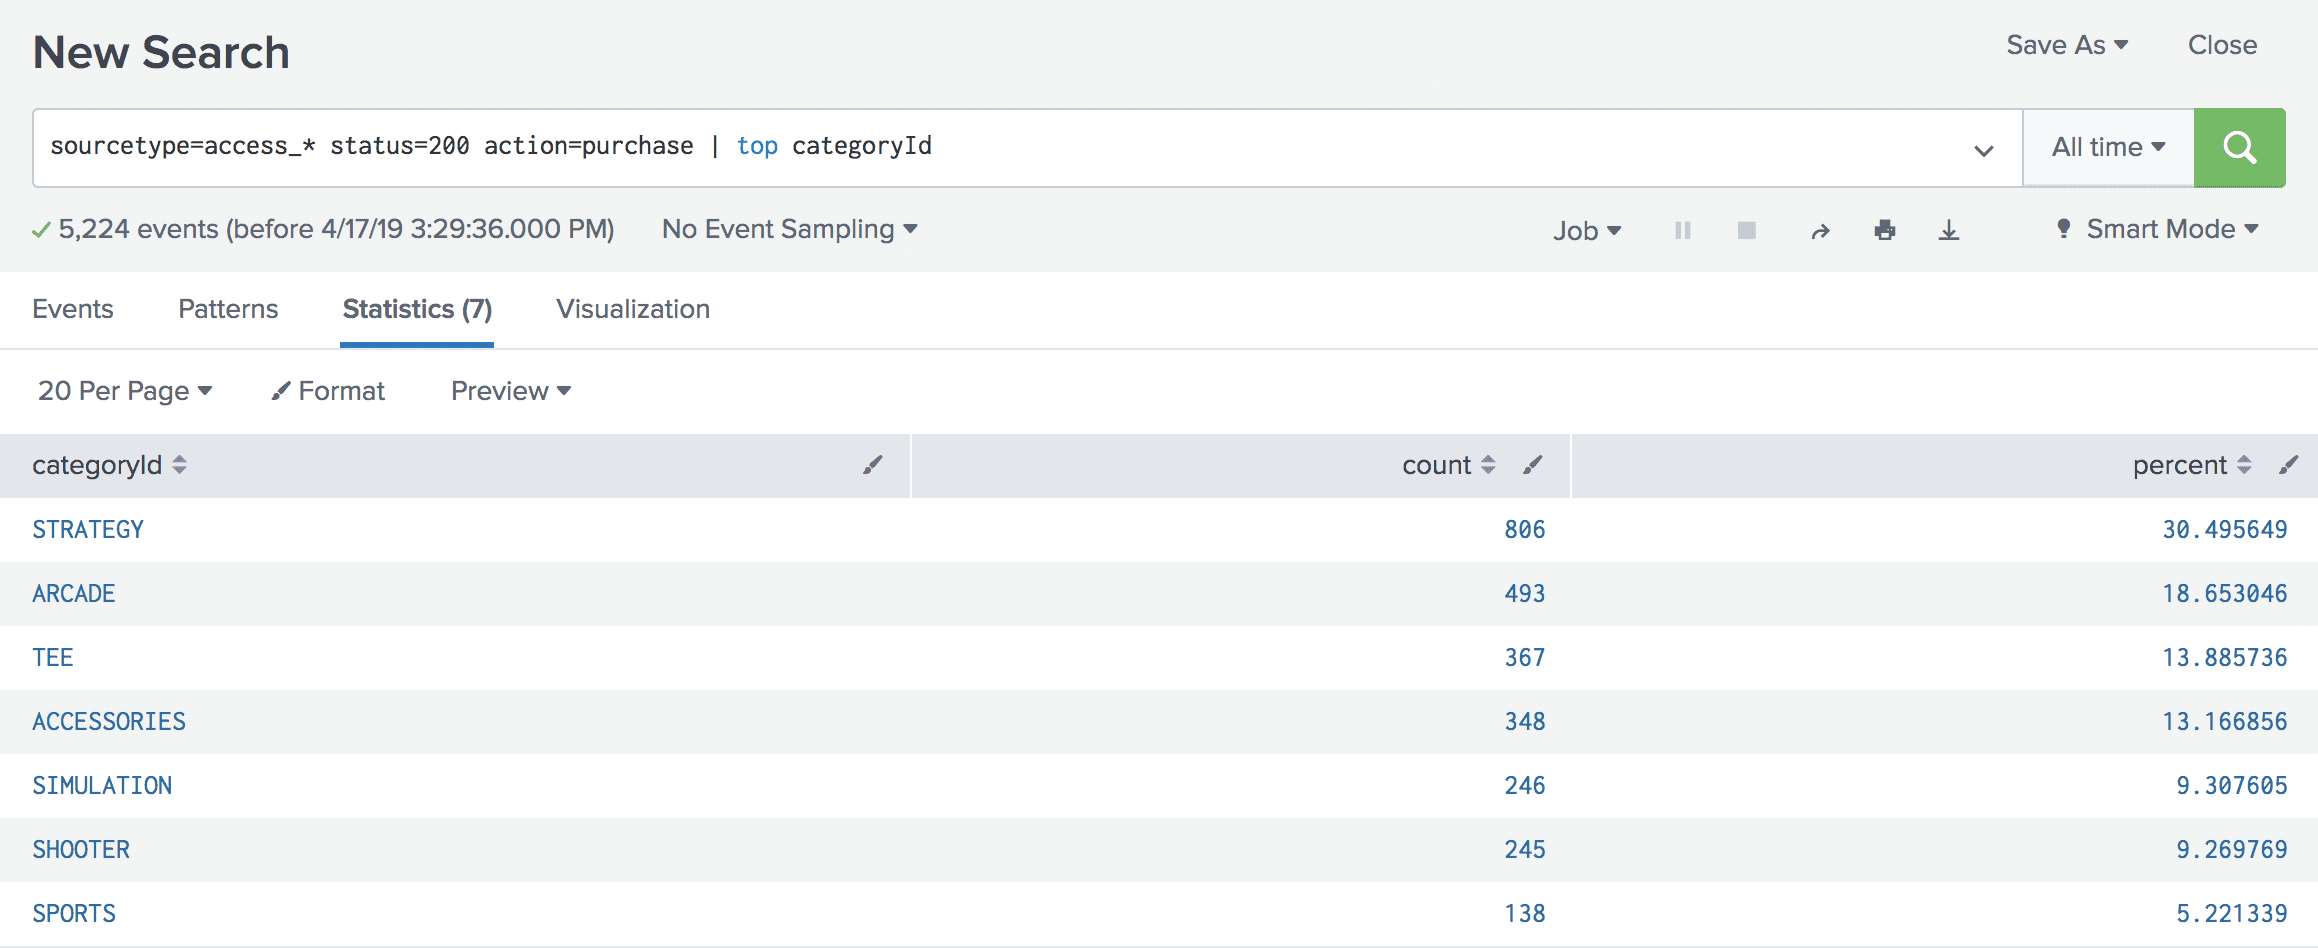
\includegraphics[width=\linewidth]{img/03_methoden/splunk_search-processing-language.png}
	\caption{Abfragebeispiel in Splunk aus \cite{SplunkSPL}}
	\label{fig:splunk_search-processing-language}
\end{figure}

\subsubsection{Jaeger}
\label{subsec:jaeger}

Jaeger wurde 2017 als ein OpenSource-Projekt der CNCF gestartet \cite{Jaeger}. Es ist ein System für verteiltes Tracing und bietet Funktionalitäten zur Datensammlung, --verarbeitung, --speicherung bis hin zur Visualisierung. Jaeger unterstützt und implementiert den Standard OpenTracing, unterstützt aber auch Datenformate anderer Hersteller (wie z. B. Zipkin \cite{Zipkin}). Eine Unterstützung des OpenTelemetry-Standards ist derzeit im Gange. Weiterhin kann Jaeger dazu benutzt werden, Metriken nach Prometheus \cite{Prometheus} zu exportieren, einem weiteren CNCF-Projekt zur Speicherung und Visualisierung von Daten.

\begin{wrapfigure}[11]{r}{0.40\textwidth}
\centering
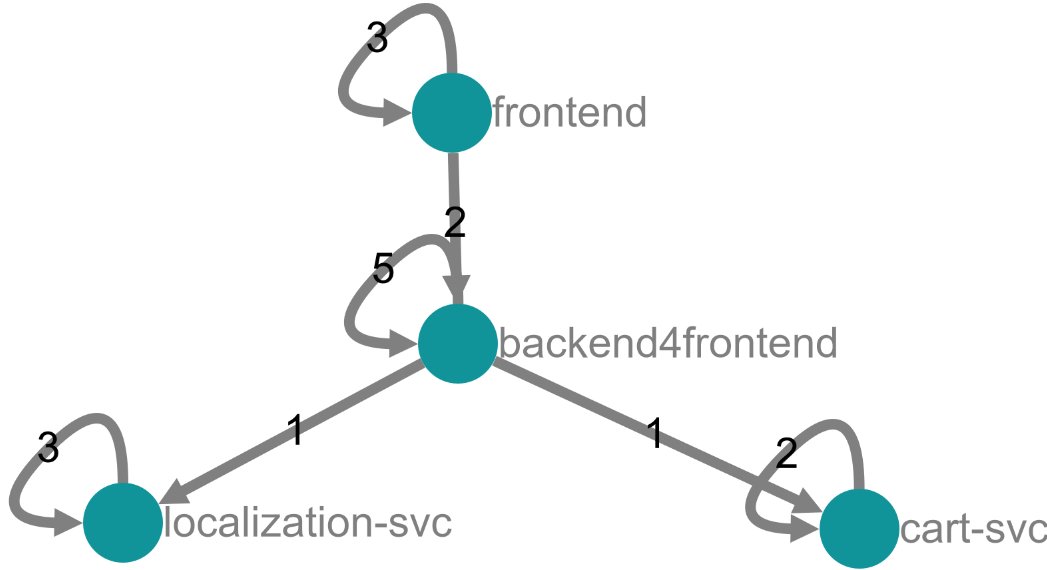
\includegraphics[width=\linewidth]{img/03_methoden/jaeger_dependency-graph.png}
\caption{Dienst-Abhängigkeits-Graph. Quelle: Eigene Darstellung}
\label{fig:jaeger-ui_dependency-graph}
\end{wrapfigure}

Jaeger spezialisiert sich auf Tracing und bietet hierfür eine skalierbare Infrastruktur zur Speicherung und Analyse der Daten. Die Traces werden als angereicherte Trace-Gantt-Diagramme dargestellt, wie in \autoref{fig:jaeger-ui_trace-detail-view} zu sehen ist. Hierbei sind sowohl hierarchische als auch zeitliche Beziehungen visualisiert. Wie bei OpenTracing und OpenTelemetry besteht ein Trace aus mehreren Spans, welche meist eine Methode umschließen. Zu den einzelnen Spans lassen sich weitere Informationen anzeigen, wenn vorhanden, wie bspw. Logmeldungen oder Kontextinformationen.

Anhand der Traces generiert Jaeger zudem automatisch eine Architektur, indem die Beziehungen zwischen Diensten zu sehen ist. In \autoref{fig:jaeger-ui_dependency-graph} kann so eine Darstellung betrachtet werden.

\begin{figure}[H]
	\centering
	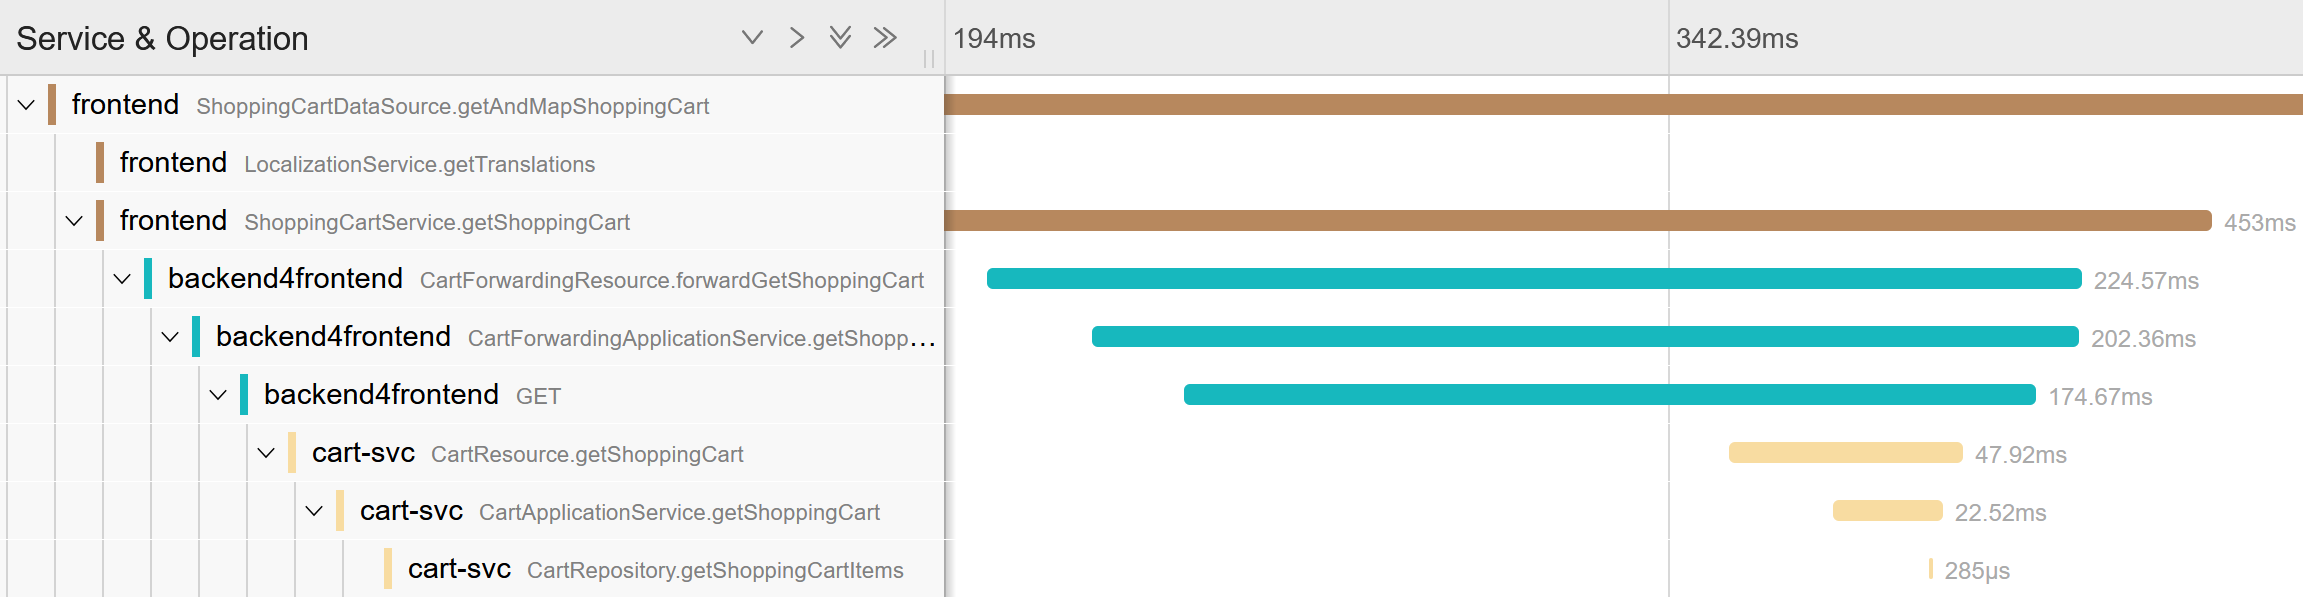
\includegraphics[width=\linewidth]{img/03_methoden/jaeger_trace-detail-view.png}
	\caption{Trace-Detailansicht. Eigener Screenshot aus Jaeger}
	\label{fig:jaeger-ui_trace-detail-view}
\end{figure}

\subsubsection{Sentry}
\label{subsec:sentry}

Sentry \cite{Sentry} ist ein SaaS-Produkt der Functional Software Inc., welches sich auf das Error Monitoring spezialisiert. Die Kernfunktionalitäten beschränken sich auf das Error Monitoring, auch wenn von anderen Praktiken einige Aspekte präsent sind, stellen diese keine eigens abgeschlossene Funktionalität dar.

Neben einer kommerziellen Version, stellt Sentry auch eine unbegrenzt kostenlos nutzbare Version bereit, welche im Rahmen dieser Arbeit evaluiert wurde. Der Quellcode für das Backend von Sentry wurde zudem veröffentlicht und bietet Sentry darüber hinaus auch eine OnPremise-Lösung, die auf Docker basiert \cite{SentrySelfHosted}. Um von Webanwendungen Fehler zu erfassen und an Sentry zu melden, bietet Sentry bei NPM \cite{NPM} quelloffene Pakete an \cite{SentryJSGithub}. Dabei werden u. A. Anbindungen für folgende Technologien bzw. Frameworks bereitgestellt: JavaScript, Angular, React und Vue.js.

Wird ein Fehler gemeldet, erstellt Sentry hierzu ein \enquote{Issue}, also einen Problembericht. In diesem Problembericht sind detaillierte Informationen zum Fehler zu finden, wie den Stacktrace, den Zeitstempel, die Nutzerumgebung (Browser, Version, etc.) und auch einen Ausschnitt der zuletzt aufgetretenen Logmeldungen in der Browserkonsole (vgl. \autoref{fig:sentry_issue-details}). Zudem schneidet Sentry jegliche Nutzerinteraktionen mit und stellt diese in dem Problembericht mit dar (vgl. \autoref{fig:sentry_issue-event-breadcrumbs}). Treten Fehler gleichen Ursprungs auf, fasst Sentry diese im selben Problembericht zusammen, jedoch kann jede einzelne Fehlerinstanz näher betrachtet werden.

Die angebotenen Fehlerinformationen von Sentry sind zahlreich und helfen beim Nachvollziehen besser als die vorher beleuchteten Werkzeuge, jedoch mangelt es an einer ganzheitlichen Nachvollziehbarkeit, d. h. wenn kein Fehlerfall eingetreten ist, bietet Sentry hierfür auch keine Informationen.

\begin{figure}[H]
	\centering
	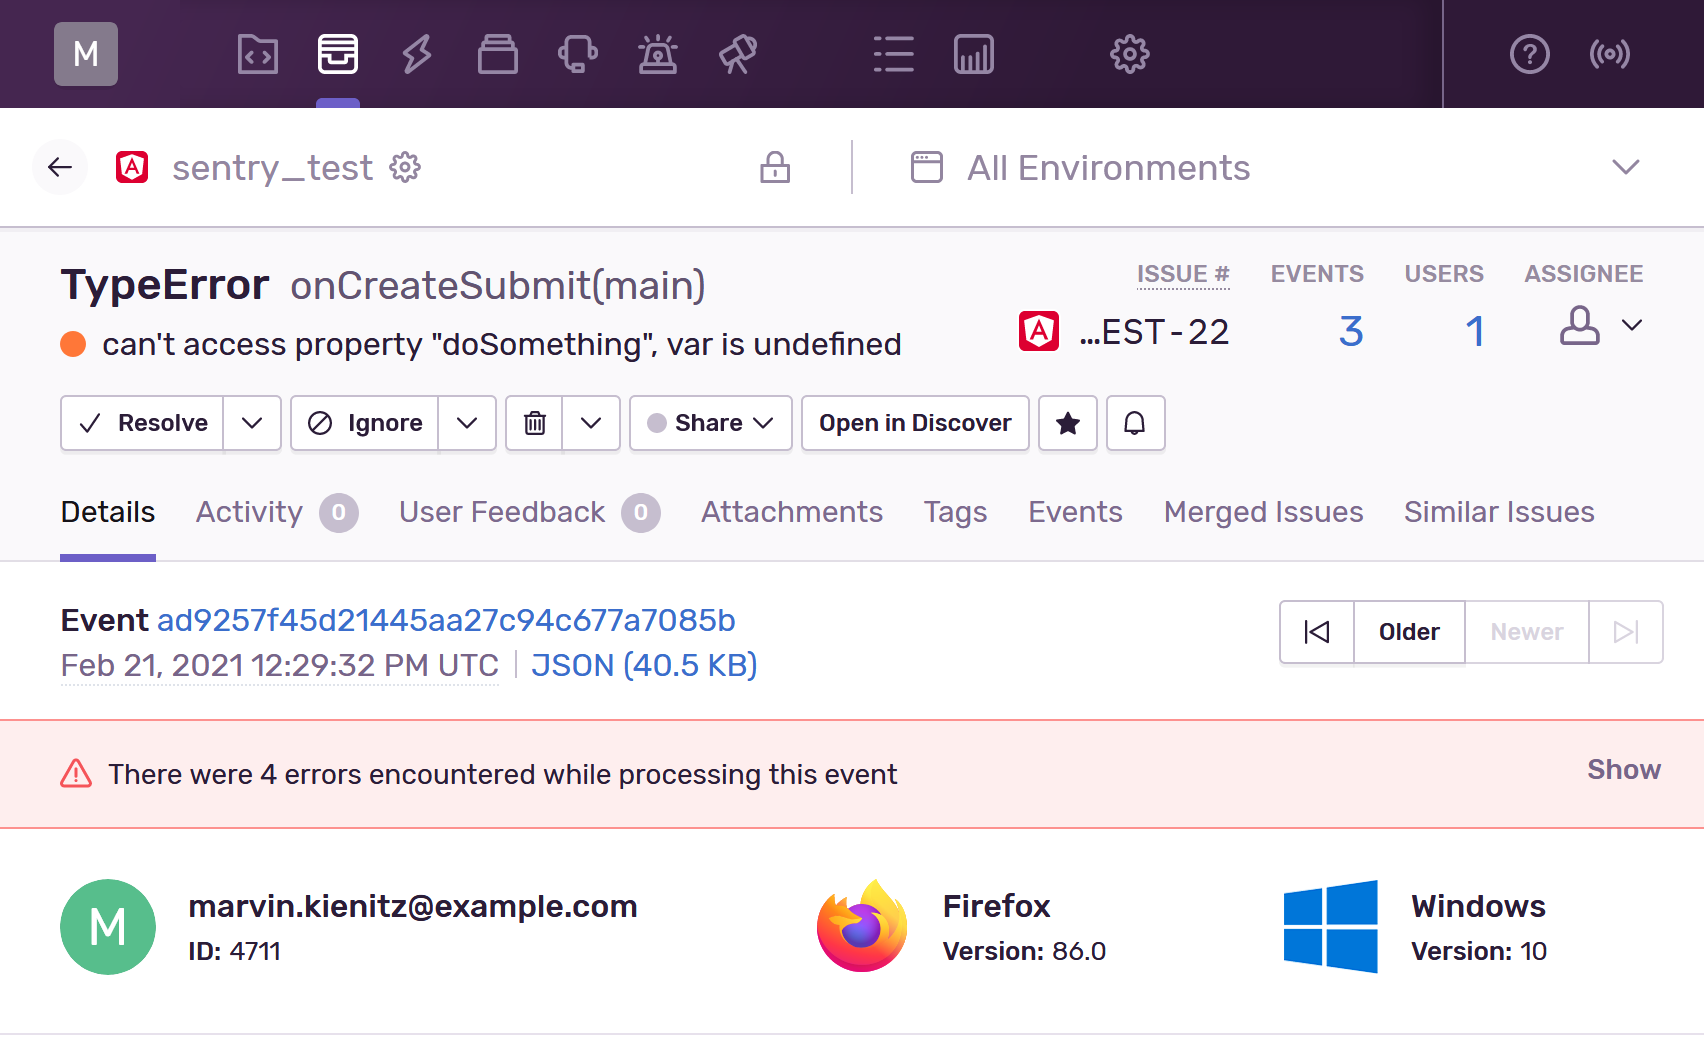
\includegraphics[width=0.9\linewidth]{img/03_methoden/sentry_issue-details.png}
	\caption{Kerninformation eines Issues. Eigener Screenshot aus Sentry}
	\label{fig:sentry_issue-details}
\end{figure}

\begin{figure}[H]
	\centering
	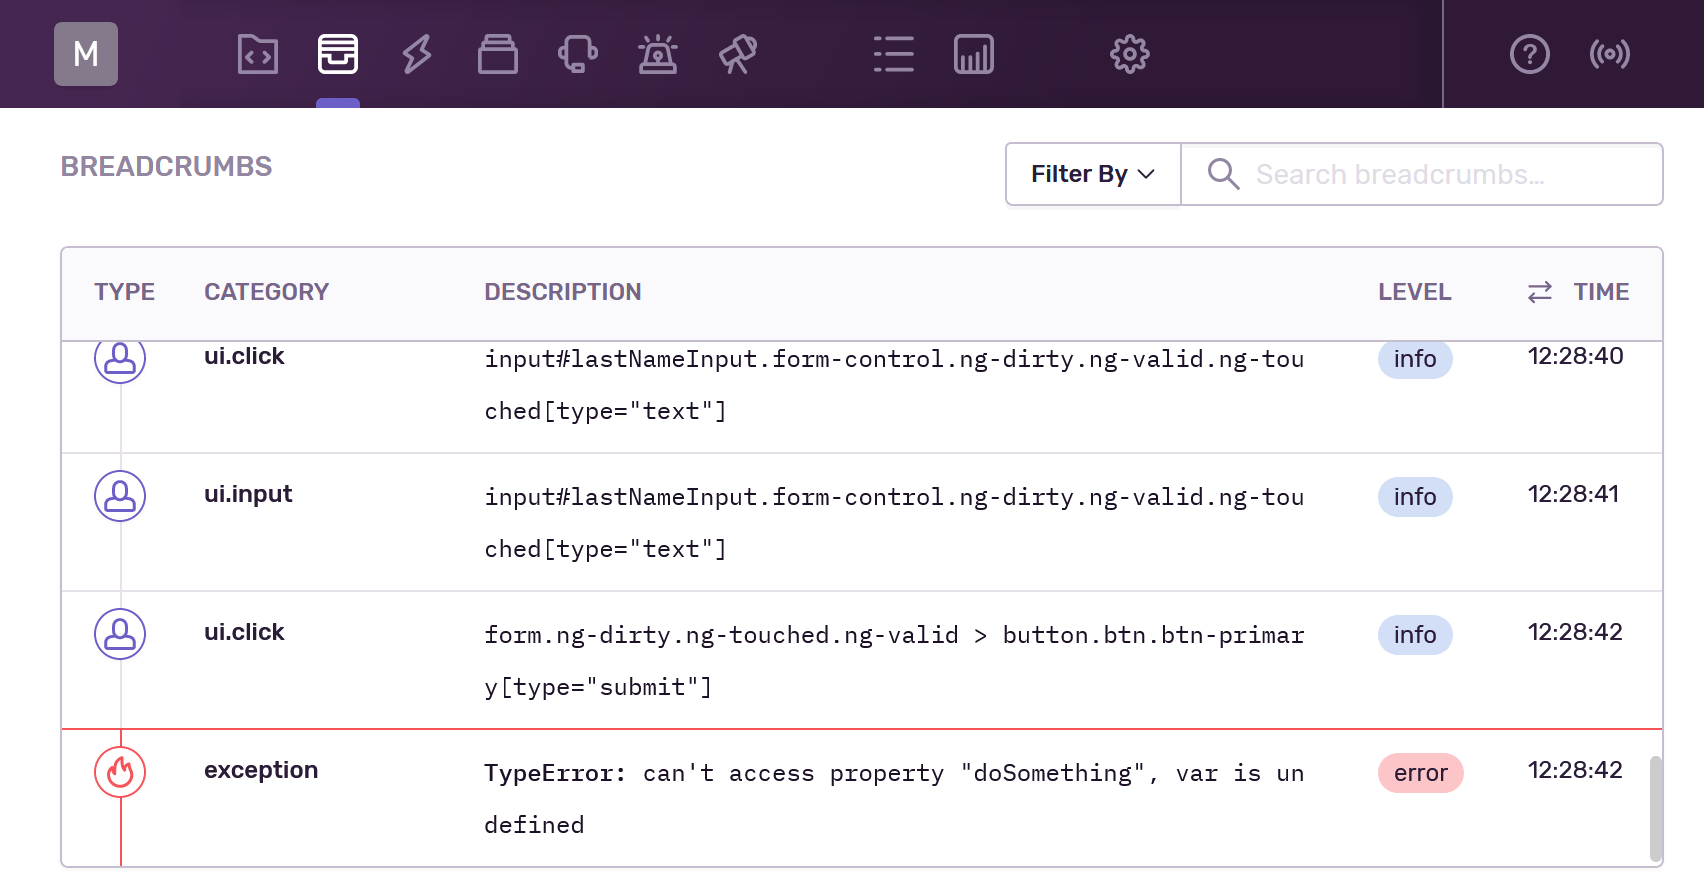
\includegraphics[width=0.80\linewidth]{img/03_methoden/sentry_issue-event-breadcrumbs.png}
	\caption{Userinteraktionen bei einer bestimmten Fehlerinstanz. Eigener Screenshot aus Sentry}
	\label{fig:sentry_issue-event-breadcrumbs}
\end{figure}

\subsubsection{LogRocket}
\label{subsec:logrocket}

LogRocket \cite{LogRocket} ist ein SaaS-Produkt des gleichnamigen Unternehmens und konzentriert sich auf detailliertes Session-Replay von JavaScript-basierten Clientanwendungen, um Probleme identifizieren, nachvollziehen und lösen zu können. Anders als vergleichbare Session-Replay-Technologien sind Entwickler die primäre Zielgruppe, nicht das Marketingteam o. Ä. \cite{Webalyt}.

LogRocket bietet eine kostenlose Testversion des SaaS-Produktes an, welche für die Evaluierung verwendet wurde. Zur Datenerhebung wird das Paket \texttt{logrocket} bei NPM angeboten, welches nach der Initialisierung eigenständig die notwendigen Daten sammelt. Mithilfe dieser Daten wird die gesamte Sitzung des Nutzers nachgestellt. Hierbei ist die Anwendung, die Nutzerinteraktionen, die Netzwerkaufrufe sowie das DOM zu sehen. Die Reproduktion wird videoähnlich aufbereitet und erlaubt ein präzises Nachvollziehen der zeitlichen Reihenfolge und Bedeutung (vgl. \autoref{fig:logrocket-session-replay-example}).

Neben dem JavaScript-SDK bietet LogRocket quelloffenene Plugins für folgende Bibliotheken: Redux, React, MobX, Vuex, ngrx, React Native. LogRocket ist zudem als OnPremise-Lösung verfügbar. Zusätzlich bietet LogRocket auch eine Integration für andere Tools, wie z. B. Sentry. Bei der Sentry-Integration wird bei einem gemeldeten Fehler direkt auf das \enquote{Video} in LogRocket verlinkt, sodass der Fehler genau betrachtet werden kann.

\begin{figure}[H]
	\centering
	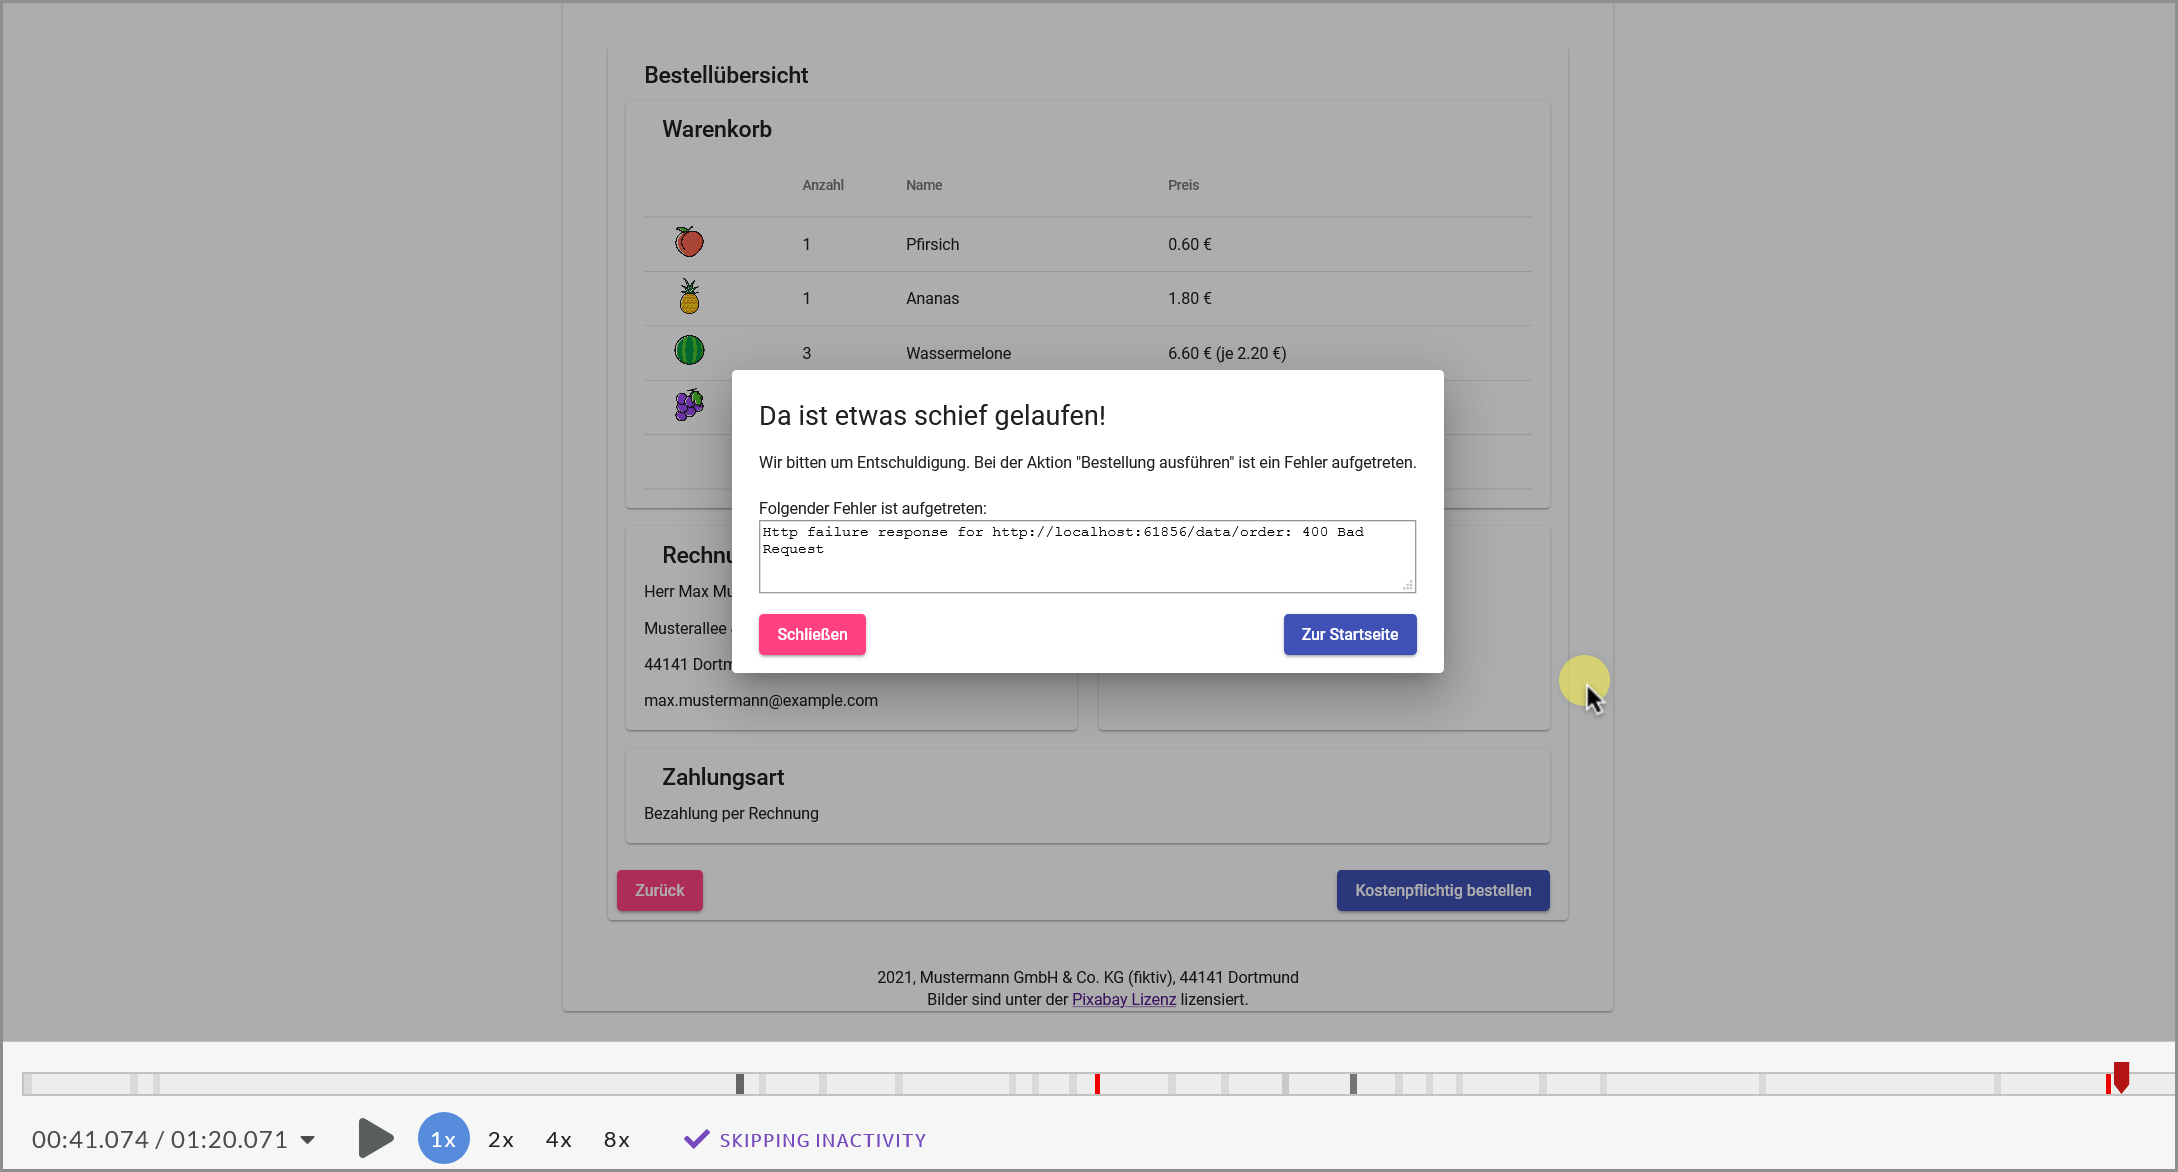
\includegraphics[width=\linewidth]{img/03_methoden/logrocket_session-replay-example-cropped.png}
	\caption{Ausschnitt eines Session Replays. Eigener Screenshot aus LogRocket}
	\label{fig:logrocket-session-replay-example}
\end{figure}

\vspace{\baselineskip}

Auf dieser Basis ist im folgenden Kapitel der eigentliche Proof-of-Concept zu entwerfen und zu implementieren. Da manche Technologien bzw. Kategorien Überschneidungen in den Funktionalitäten vorweisen (bspw. Splunk und Sentry), kommt es ggf. dazu, dass nicht alle hier identifizierten Technologien im Proof-of-Concept zum Einsatz kommen. Vor dem Proof-of-Concept wird jedoch zunächst die die Demoanwendung, auf der das Konzept angewendet werden soll, vorgestellt.